\documentclass[11pt,letterpaper]{article}
\usepackage{fullpage}
\usepackage[top=2cm, bottom=4.5cm, left=2.5cm, right=2.5cm]{geometry}
\usepackage{amsmath,amsfonts,amssymb}
\usepackage{lastpage}
\usepackage[inline]{enumitem}
\usepackage{fancyhdr}
\usepackage{mathrsfs}
\usepackage{xcolor}
\usepackage{graphicx}
\usepackage{hyperref}
\hypersetup{colorlinks=true, linkcolor=blue, linkbordercolor={0 0 1}}

\renewcommand{\arraystretch}{1.75}

\newcommand{\qrf}{\texttt{QRFactor}}

\setlength{\parindent}{0.0in}
\setlength{\parskip}{0.05in}

\pagestyle{fancyplain}
\lhead{Brad Cownden}
\chead{}
\rhead{April 2, 2020}
\cfoot{\small\thepage}
\headsep 36pt

\begin{document}

This document will outline the settings and libraries required to build and execute QRFactor in either Visual Studio or Nsight Eclipse. It is assumed that the \href{https://developer.nvidia.com/cuda-downloads}{CUDA Toolkit} (which includes Nsight Eclipse) has already been installed, as well \href{https://visualstudio.microsoft.com/downloads/}{Microsoft Visual Studio} if required. The read-in of the system matrix $A$ requires the data to be in Matrix Market format (see the \href{https://math.nist.gov/MatrixMarket/formats.html}{NIST page} for more information on MMF, as well as to download the library routines \texttt{mmio.h} and \texttt{mmio.c}).

\section{Running \texttt{QRFactor} in Visual Studio 2019 (VS2019)}
\label{sec: vs}

Place the system matrix file \texttt{sysMatA.mtx}, the library routines \texttt{mmio.c} and \texttt{mmio.h}, the wrapper \texttt{mmio\_wrapper.cpp}, the source file \texttt{QRFactor.cpp}, and the VS2019 files \texttt{QRFactor.vcxproj} and \texttt{QRFactor.vcxproj.user} in a single directory. The time-dependent input data files can be located in a separate directory that will be set later.

There are several project settings that will need to be changed before the program can be built. These will be discussed below, and screen shots of the relevant settings will be included in appendix~\ref{app: VS settings}. The following settings will ensure that VS2019 is able to find the correct library files:
\begin{itemize}
\item Under Advanced Properties, ensure {\bf MSVC Toolset} is set to 14.25.28610.
\item Under C++/General, ensure {\bf Additional Include Directories} contains ./;\$(CudaToolkitIncludeDir);\$(CudaToolkitIncludeDir)/include;C:/ProgramData/NVIDIA Corporation/CUDA Samples/v10.2/common/inc.
\item Under C++/Optimization, ensure {\bf Optimization} is set to Maximum Optimization (Favour Speed) (/O2).
\item Under Linker/General, ensure {\bf Additional Library Directories} is set to \$(CudaToolitLibDir).
\item Under Linker/Input, ensure {\bf Additional Dependencies} includes cusolver.lib;cusparse.lib; cudart\_static.lib;kernel32.lib;user32.lib;gdi32.lib;winspool.lib;comdlg32.lib;advapi32.lib; \\ shell32.lib;ole32.lib;oleaut32.lib;uuid.lib;odbc32.lib;odbccp32.lib;\%(AdditionalDependencies).
\end{itemize}

With these settings in place, the project can be built by selecting Build $\to$ Build QRFactor (Ctrl + B). \texttt{QRFactor.exe} can then be run either through VS2019 or via the command line.

\section{Running \texttt{QRFactor} in Nsight Eclipse}
\label{sec: nsight}

%%%%%%%%%%%%%%%%%%%%%%%%%%%%%%%%%%%%%%%%%%%%%%%%%%%%%%%%%%%%%%%%%%%%%%%%%%%%%%
%%%%%%%%%%%%%%%%%%%%%%%%%%%%%%%%%%%%%%%%%%%%%%%%%%%%%%%%%%%%%%%%%%%%%%%%%%%%%%

\appendix

\section{Visual Studio Settings}
\label{app: VS settings}

\begin{figure}[h]
  \centering
  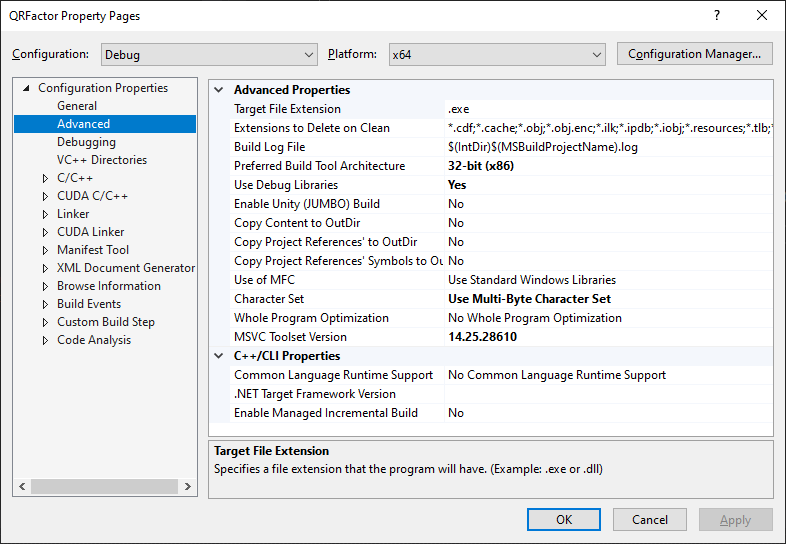
\includegraphics[width=0.7\textwidth]{C:/Users/bradc/Documents/MHI/Output/ConfigProperties_Advanced}
  \label{f: configproperties_advanced}
  \caption{QRFactor Properties $\to$ Advanced}
\end{figure}

\begin{figure}[h]
  \centering
  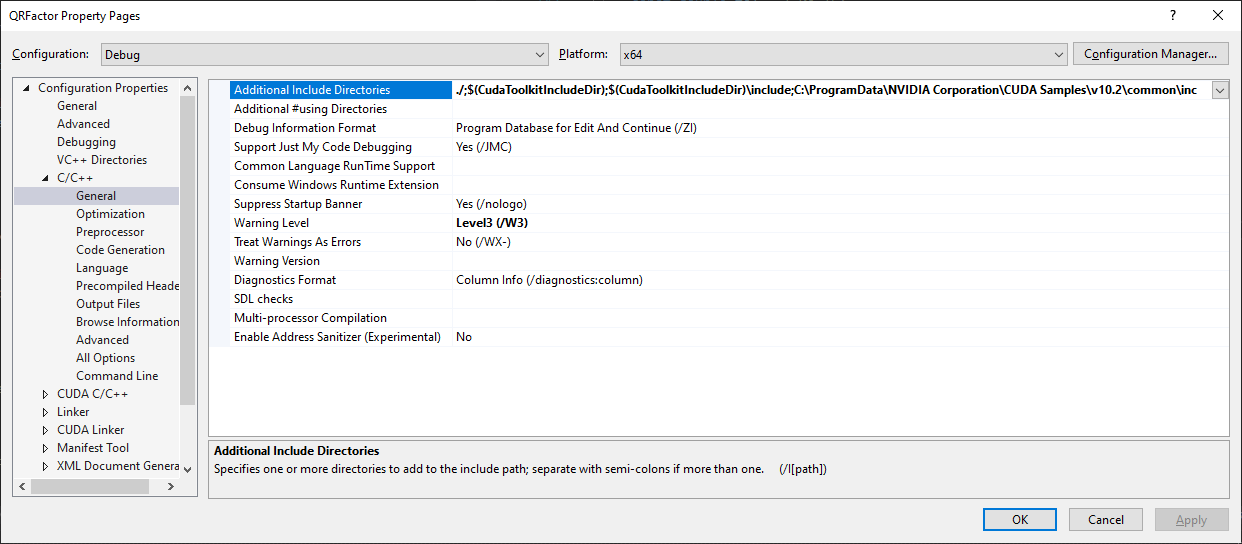
\includegraphics[width=0.7\textwidth]{C:/Users/bradc/Documents/MHI/Output/CplusplusProperites_General}
  \caption{QRFactor Properties $\to$ C/C$++$ $\to$ General}
\end{figure}

\begin{figure}[h]
  \centering
  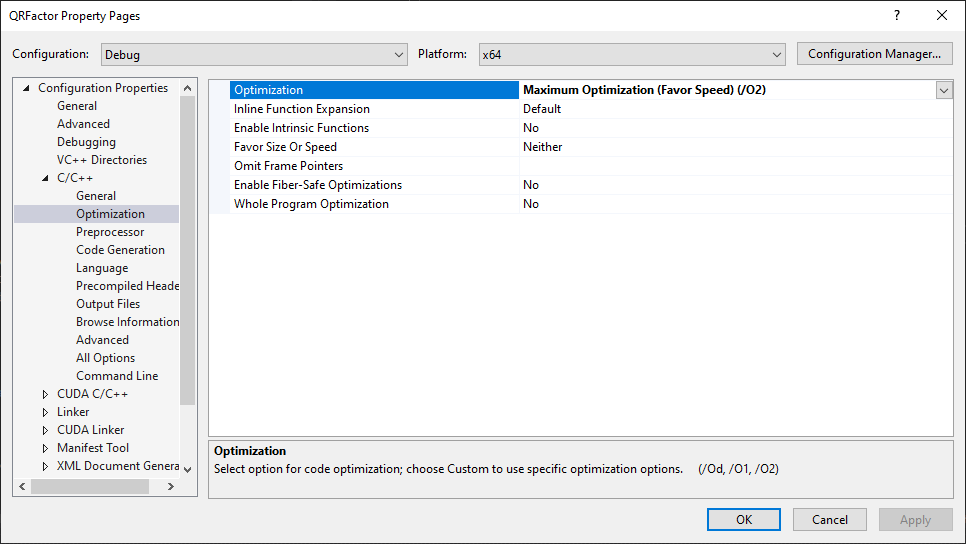
\includegraphics[width=0.7\textwidth]{C:/Users/bradc/Documents/MHI/Output/CplusplusProperites_Optimization}
  \caption{QRFactor Properties $\to$ C/C$++$ $\to$ Optimization}
\end{figure}

\begin{figure}[h]
  \centering
  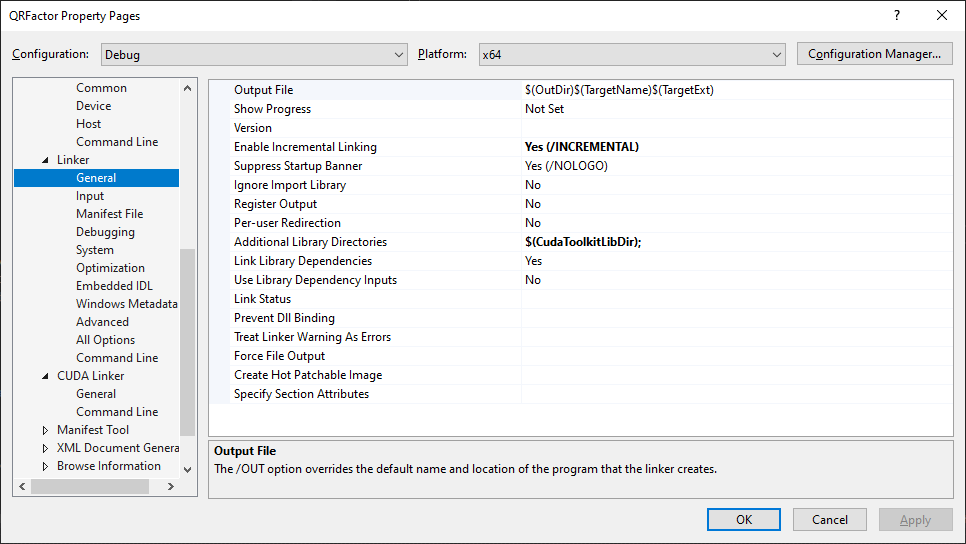
\includegraphics[width=0.7\textwidth]{C:/Users/bradc/Documents/MHI/Output/Linker_General}
  \caption{QRFactor Properties $\to$ Linker $\to$ General}
\end{figure}

\begin{figure}[h]
  \centering
  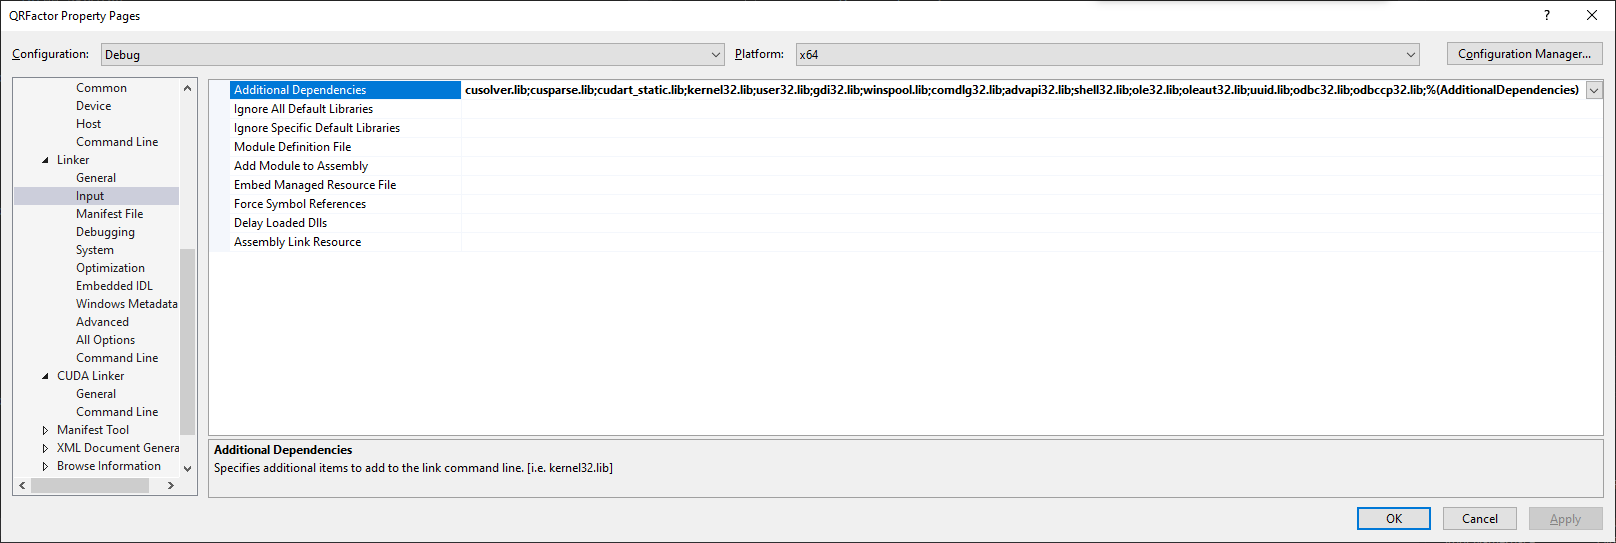
\includegraphics[width=0.7\textwidth]{C:/Users/bradc/Documents/MHI/Output/Linker_Input}
  \caption{QRFactor Properties $\to$ Linker $\to$ Input}
\end{figure}
































\end{document}
